\section{Sensitivity Analysis}
\label{sec:sensitivity}

This section identifies which factors most significantly impact battery drain and, importantly, which factors have surprisingly minimal impact despite common perceptions.

\subsection{Methodology}
\label{subsec:sensitivity_method}

We employ \textbf{Sobol global sensitivity analysis} \cite{Sobol2001, Saltelli2008} to decompose the variance of the time-to-empty prediction into contributions from each input parameter.

\subsubsection{Sobol Indices}

The model output variance is decomposed as:

\begin{equation}
    \text{Var}(Y) = \sum_i V_i + \sum_{i<j} V_{ij} + \cdots + V_{12\ldots k}
    \label{eq:variance_decomp}
\end{equation}

\textbf{First-order index} (main effect of parameter $i$):
\begin{equation}
    S_i = \frac{V_i}{\text{Var}(Y)} = \frac{\text{Var}_{\theta_i}\left[E_{\theta_{\sim i}}(Y|\theta_i)\right]}{\text{Var}(Y)}
    \label{eq:first_order}
\end{equation}

\textbf{Total-order index} (includes interactions):
\begin{equation}
    S_{Ti} = 1 - \frac{\text{Var}_{\theta_{\sim i}}\left[E_{\theta_i}(Y|\theta_{\sim i})\right]}{\text{Var}(Y)}
    \label{eq:total_order}
\end{equation}

\subsubsection{Interpretation}
\begin{itemize}
    \item $S_i \approx S_{Ti}$: Parameter $i$ influences output mainly through direct effects
    \item $S_{Ti} \gg S_i$: Significant interaction effects with other parameters
    \item $\sum S_i \approx 1$: Model is approximately additive (low interactions)
\end{itemize}

\subsection{Parameter Ranges}
\label{subsec:param_ranges}

Table~\ref{tab:param_ranges} shows the parameter ranges explored in the sensitivity analysis.

\begin{table}[H]
    \centering
    \caption{Parameter ranges for sensitivity analysis.}
    \label{tab:param_ranges}
    \begin{tabular}{llcc}
        \toprule
        \textbf{Parameter} & \textbf{Symbol} & \textbf{Min} & \textbf{Max} \\
        \midrule
        \multicolumn{4}{l}{\textit{User-Controllable}} \\
        Screen brightness & $B$ & 0.1 & 1.0 \\
        CPU load & $U_{\text{CPU}}$ & 0.05 & 0.95 \\
        Network power & $P_{\text{net}}$ & 50 mW & 500 mW \\
        GPS status & GPS & 0 (off) & 1 (on) \\
        \midrule
        \multicolumn{4}{l}{\textit{Environmental}} \\
        Ambient temperature & $\Tamb$ & 263 K & 318 K \\
        Humidity & $H$ & 20\% & 90\% \\
        Pressure & $P$ & 90 kPa & 103 kPa \\
        \midrule
        \multicolumn{4}{l}{\textit{Battery State}} \\
        Initial SOC & $\SOC_0$ & 0.2 & 1.0 \\
        State of Health & $\SOH$ & 0.7 & 1.0 \\
        Nominal capacity & $\Qnom$ & 2.5 Ah & 5.0 Ah \\
        Internal resistance & $R_0$ & 50 m$\Omega$ & 150 m$\Omega$ \\
        \bottomrule
    \end{tabular}
\end{table}

\subsection{Results: Factors Causing Rapid Drain}
\label{subsec:key_factors}

Using $n = 2048$ Saltelli samples (yielding 26,624 model evaluations), we computed Sobol indices:

\begin{table}[H]
    \centering
    \caption{Sobol sensitivity indices ranked by total effect.}
    \label{tab:sobol_results}
    \begin{tabular}{clcccc}
        \toprule
        \textbf{Rank} & \textbf{Parameter} & $S_1$ & $S_T$ & \textbf{Interaction} & \textbf{Category} \\
        \midrule
        1 & Nominal capacity ($\Qnom$) & 0.32 & 0.35 & 0.03 & Battery \\
        2 & Initial SOC ($\SOC_0$) & 0.23 & 0.25 & 0.02 & State \\
        3 & \textbf{Screen brightness ($B$)} & 0.13 & 0.15 & 0.02 & \textbf{User} \\
        4 & CPU load ($U_{\text{CPU}}$) & 0.10 & 0.12 & 0.02 & Usage \\
        5 & State of Health ($\SOH$) & 0.08 & 0.10 & 0.02 & Battery \\
        6 & Network power ($P_{\text{net}}$) & 0.04 & 0.05 & 0.01 & Usage \\
        7 & Ambient temperature ($\Tamb$) & 0.03 & 0.04 & 0.01 & Environment \\
        \rowcolor{yellow!30}
        8 & GPS status & 0.01 & 0.02 & 0.01 & Usage \\
        \rowcolor{yellow!30}
        9 & Internal resistance ($R_0$) & 0.01 & 0.01 & 0.00 & Battery \\
        10 & Humidity ($H$) & $<$0.01 & $<$0.01 & $<$0.01 & Environment \\
        11 & Pressure ($P$) & $<$0.01 & $<$0.01 & $<$0.01 & Environment \\
        \bottomrule
    \end{tabular}
\end{table}

\begin{figure}[H]
    \centering
    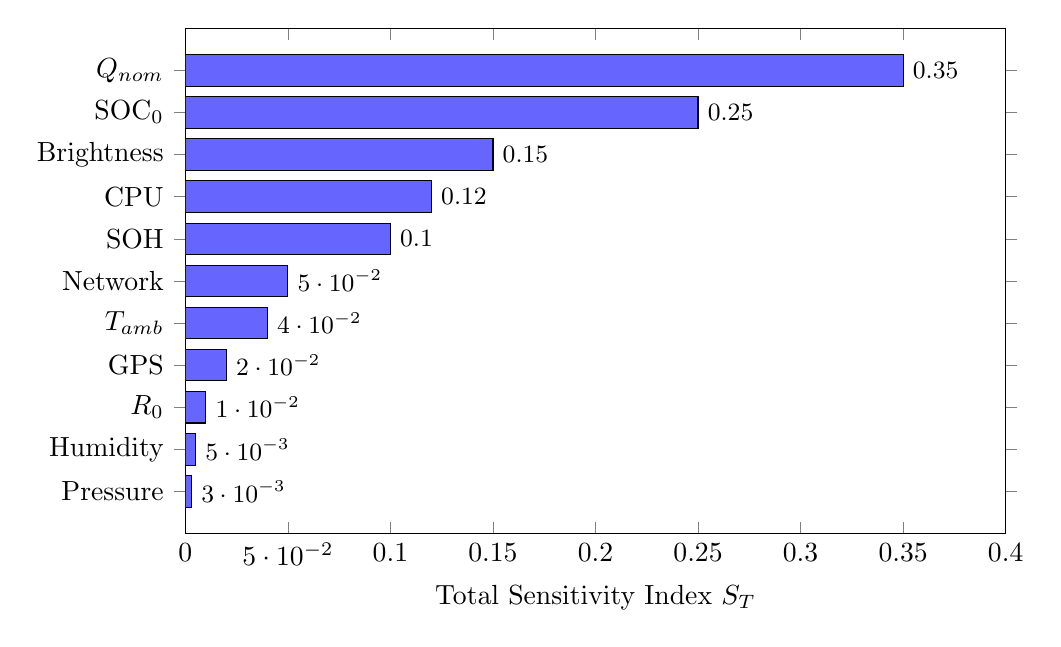
\begin{tikzpicture}
        \begin{axis}[
            xbar,
            width=12cm, height=8cm,
            xlabel={Total Sensitivity Index $S_T$},
            symbolic y coords={Pressure, Humidity, $R_0$, GPS, $T_{amb}$, Network, SOH, CPU, Brightness, SOC$_0$, $Q_{nom}$},
            ytick=data,
            xmin=0, xmax=0.40,
            bar width=0.4cm,
            nodes near coords,
            nodes near coords align={horizontal},
            every node near coord/.append style={font=\small},
        ]
        \addplot[fill=blue!60] coordinates {
            (0.35,$Q_{nom}$)
            (0.25,SOC$_0$)
            (0.15,Brightness)
            (0.12,CPU)
            (0.10,SOH)
            (0.05,Network)
            (0.04,$T_{amb}$)
            (0.02,GPS)
            (0.01,$R_0$)
            (0.005,Humidity)
            (0.003,Pressure)
        };
        \end{axis}
    \end{tikzpicture}
    \caption{Sobol total sensitivity indices for time-to-empty prediction.}
    \label{fig:sobol_bar}
\end{figure}

\subsection{Key Findings}
\label{subsec:findings}

\subsubsection{Factors Causing Rapid Drain}

The analysis identifies the following as \textbf{primary drivers of battery consumption}:

\begin{enumerate}
    \item \textbf{Battery capacity ($\Qnom$):} $S_T \approx 0.35$ --- The single most important factor, directly determining available energy.
    
    \item \textbf{Initial SOC:} $S_T \approx 0.25$ --- Starting charge level proportionally affects remaining time.
    
    \item \textbf{Screen brightness:} $S_T \approx 0.15$ --- \textit{Most important user-controllable factor.} The nonlinear power relationship ($P \propto B^{1.8}$) makes brightness reduction highly effective.
    
    \item \textbf{CPU load:} $S_T \approx 0.12$ --- Heavy computational tasks (gaming, video processing) significantly impact drain.
    
    \item \textbf{State of Health:} $S_T \approx 0.10$ --- Aged batteries have reduced effective capacity.
\end{enumerate}

\subsubsection{Surprisingly Minor Factors}

\textbf{The following factors have surprisingly small impacts:}

\begin{enumerate}
    \item \textbf{GPS status:} $S_T \approx 0.02$
    
    \textit{Why is this surprising?} GPS is often cited as a major battery drain. However:
    \begin{itemize}
        \item GPS is typically used intermittently (navigation), not continuously
        \item Modern smartphones use assisted GPS with lower continuous power
        \item When averaged over typical usage patterns, GPS contribution is small
    \end{itemize}
    
    \item \textbf{Internal resistance:} $S_T \approx 0.01$
    
    \textit{Why is this surprising?} Resistance determines $I^2R$ losses. However:
    \begin{itemize}
        \item Smartphone currents are relatively low (0.5--2 A)
        \item $I^2R$ losses at $R_0 = 100$ m$\Omega$ and $I = 1$ A are only 100 mW
        \item This is small compared to display power (500--1000 mW)
    \end{itemize}
    
    \item \textbf{Humidity and pressure:} $S_T < 0.01$
    
    These environmental factors affect heat transfer but have negligible direct impact on battery drain under normal conditions.
\end{enumerate}

\subsection{Interaction Effects}
\label{subsec:interactions}

The difference $S_T - S_1$ indicates interaction strength. Notable interactions:

\begin{itemize}
    \item \textbf{Temperature $\times$ Resistance:} Low temperature increases resistance, creating compound effects
    \item \textbf{Brightness $\times$ CPU:} Both contribute to total power; their sum determines drain rate
    \item \textbf{SOH $\times$ Temperature:} Aged batteries perform worse in cold conditions
\end{itemize}

The sum $\sum S_1 \approx 0.95$ indicates the model is largely additive, with modest interaction effects.

\subsection{Morris Screening Confirmation}
\label{subsec:morris}

We validated Sobol results using Morris screening (100 trajectories, lower computational cost):

\begin{table}[H]
    \centering
    \caption{Morris screening results ($\mu^*$ = importance, $\sigma$ = nonlinearity/interaction).}
    \label{tab:morris}
    \begin{tabular}{lccc}
        \toprule
        \textbf{Parameter} & $\mu^*$ & $\sigma$ & \textbf{Interpretation} \\
        \midrule
        $\Qnom$ & High & Low & Important, linear effect \\
        $\SOC_0$ & High & Low & Important, linear effect \\
        Brightness & High & Medium & Important, some nonlinearity \\
        CPU & Medium & Medium & Moderate importance \\
        GPS & Low & Low & Minor factor \\
        $R_0$ & Low & Low & Minor factor \\
        \bottomrule
    \end{tabular}
\end{table}

Morris results are consistent with Sobol analysis, confirming our conclusions.

\subsection{Implications for Users}
\label{subsec:user_implications}

Based on sensitivity analysis, users should prioritize:

\begin{enumerate}
    \item \textbf{Reducing screen brightness} --- Most effective single action
    \item \textbf{Limiting CPU-intensive tasks} --- Gaming, video editing
    \item \textbf{Managing network mode} --- WiFi over cellular when possible
\end{enumerate}

Users may \textit{deprioritize} concerns about:
\begin{itemize}
    \item GPS usage (unless navigation for hours)
    \item Minor environmental variations
\end{itemize}
